\documentclass[runningheads]{llncs}

\usepackage[T1]{fontenc}
\usepackage[utf8]{inputenc}
\usepackage{graphicx}
\usepackage{amsmath}
\usepackage{amssymb}
\usepackage{booktabs}
\graphicspath{{techniques/reusable-format/jpeg/out/}}
\usepackage{listings}
\usepackage{xcolor}
\usepackage{adjustbox}
% nota: colores para los bloques de codigo
\definecolor{codebg}{RGB}{248,248,248}
\definecolor{codeframe}{RGB}{220,220,220}
\definecolor{codegray}{gray}{0.45}
\lstdefinestyle{code}{
    basicstyle=\ttfamily\footnotesize,
    backgroundcolor=\color{codebg},
    frame=single, rulecolor=\color{codeframe},
    columns=fullflexible, keepspaces=true,
    showstringspaces=false,
    breaklines=true, breakatwhitespace=false,
    numbers=left, numberstyle=\tiny\color{codegray},
    xleftmargin=1.5em
}
\lstdefinestyle{console}{style=code, language=bash}
\lstdefinestyle{python}{style=code, language=Python}
% hex/plain text dumps
\lstdefinestyle{textblock}{style=code, language={} }
% inline highlighting with @...@
\lstdefinestyle{hexhi}{
    style=textblock,
    moredelim=**[is][\bfseries\color{red}]{@}{@}
}

\lstdefinestyle{textblock}{%
    basicstyle=\ttfamily\footnotesize,
    columns=fullflexible,
    keepspaces=true,
    breaklines=false,
    numbers=none,
    frame=single,
}

\lstdefinestyle{hashblock}{%
    basicstyle=\ttfamily\footnotesize,
    columns=fullflexible,
    keepspaces=true,
    breaklines=true,
    numbers=none,
    frame=single,
}

\lstdefinestyle{hexhi}{%
    basicstyle=\ttfamily\scriptsize,
    columns=fullflexible,
    keepspaces=true,
    breaklines=false,
    numbers=none,
    frame=single,
% highlight @..@ spans
    literate={@}{}1
        {@00@}{{\bfseries\color{red}00}}3
        {@01@}{{\bfseries\color{red}01}}3
        {@24@}{{\bfseries\color{red}24}}3
        {@25@}{{\bfseries\color{red}25}}3
}


\usepackage{url}
\usepackage{hyperref}
\usepackage{pdfpages}
\hypersetup{
    colorlinks=true,
    linkcolor=blue,
    filecolor=magenta,
    urlcolor=cyan,
}
\def\UrlBreaks{\do\/\do-}

\begin{document}

    \title{Practical Collision Attacks on the MD5 Hash Function}
    \titlerunning{Practical Collision Attacks on MD5}
    \author{Alfonso Pedro Ridao (s243942) \and Martina Siderini (s252978) \and Ayiyuh Ambe Che (s243440)}
    \authorrunning{A. P. Ridao, M. Siderini, and A. A. Che}

    \institute{Technical University of Denmark (DTU)}
    \maketitle

    \begin{abstract}
        This report examines vulnerabilities in cryptographic hash functions, with a specific focus on the MD5 algorithm. We explain the theory behind collision attacks, show their practical security threats using real-world examples, and classify different types of related attacks. This background information is used to support a series of hands-on experiments that demonstrate identical-prefix, chosen-prefix, and reusable collision attacks.
        \keywords{MD5 \and Hash Collision \and Cryptanalysis \and Data Integrity}
    \end{abstract}

    \section{Introduction: Cryptographic Hashes and Collision Attacks}

    A cryptographic hash function is an algorithm that takes an input of any size and produces a fixed-size output. This output is usually called a digest or a hash value. The digest works like a unique "fingerprint" for the original data. If any part of the input is changed, even just a single bit, the hash output should change completely. This is known as the \textbf{avalanche effect}.

    Hash functions are designed to have two main security properties. They are one-way, which means it is not practical to figure out the original input from its hash. They are also collision-resistant, meaning it is extremely difficult to find two different inputs that create the same hash (NIST NVD, 2009). These properties are essential for protecting data integrity. For example, the \textbf{MD5 algorithm} was created to be a secure tool for digital signatures and for verifying that files have not been altered (Rivest, 1992).

    The security of a hash function fully depends on its collision resistance. According to a mathematical concept called the pigeonhole principle, collisions must exist. However, a secure hash function makes the work of finding a collision practically impossible. For a perfect hash with an n-bit output, a brute-force search for a collision would require about $2^{n/2}$ operations. This estimate comes from the \textbf{birthday paradox}. For a 128-bit hash like MD5, this would be $2^{64}$ operations.

    Unfortunately, major weaknesses were found in MD5’s design. These flaws allowed cryptanalysts to find collisions much more easily. By 2006, the attacks had become so advanced that an MD5 collision could be generated in under a minute on a regular laptop computer (Klima, 2006).


    \section{The Security Threat of MD5 Collisions}

    In cryptography, a collision attack is a method for finding two different inputs, M and M’, that produce the exact same hash output, so that $H(M) = H(M')$, even though $M \neq M'$ (Leurent and Peyrin, 2020).

    The ability to intentionally create hash collisions is a serious security threat. If an attacker can make two different files with the same hash, they can trick systems that use hashes to verify trust. The classic example is a digital signature. A signature is created validating the hash of a document, not the actual document itself. An attacker can create a harmless document (A) and a malicious document (B) that both share the same hash. The attacker then gets the harmless document A officially signed. Because the signature is just for the hash, they can take that signature and attach it to the malicious document B. The signature will appear valid because the hash it belongs to has not changed (Stevens, Lenstra and de Weger, 2012; \cite{microsoft}).

    This is not just a theoretical problem. There are real-world examples. Researchers created two different X.509 SSL certificates that had the same MD5 hash. One was for a legitimate website, but the other was for a fake Certificate Authority (CA). Because the hashes matched, the fake certificate could be trusted (Stevens et al., 2009; \cite{microsoft}). Additionally, the "Flame" malware found in 2012 used a new type of chosen-prefix collision attack. This attack allowed it to fake a Microsoft code-signing certificate, which made its malicious code look like authentic software from Microsoft (Fillinger and Stevens, 2015).

    These incidents show that once a hash function's collision resistance is broken, it must be considered unsafe and should no longer be used for security purposes (\cite{microsoft}).

    \paragraph{Threat Model and Realistic Scenario.}
    \textbf{Adversary.} An external attacker can generate MD5 identical- or chosen-prefix collisions offline and can submit benign-looking content to be signed, whitelisted, or distributed. The attacker cannot break public-key signatures or tamper with servers after publication. \textbf{Targets.} (i) Enterprise email gateways and DLP systems that trust MD5 for attachment de-duplication or policy decisions; (ii) software allow-lists and vendor update feeds that identify binaries by MD5; (iii) document workflows where the signature or approval is bound to an MD5 of a PDF rather than to a canonicalized document object.

    \textbf{Scenario.} The attacker crafts two files with the \emph{same} MD5: a benign “cover” object that is submitted for approval/signing/allow-listing, and a malicious counterpart. In a chosen-prefix setting, two different preambles (e.g., invoice vs.\ wire-instruction PDF headers or two DER-encoded CSRs) are linked with tailored suffixes so their full-file MD5 digests collide. In a reusable-collision setting, a short collided prefix plus a large identical suffix yields two files that render or unpack \emph{different} content while hashing identically. After the benign object is approved (signature attached, hash added to an allow-list, or update feed published), the attacker substitutes the malicious twin: verification that relies on MD5 alone accepts it as legitimate, enabling document fraud, policy bypass, or malicious code distribution.

    \textbf{Security impact.} Integrity and non-repudiation guarantees collapse wherever MD5 is the trust anchor; downstream systems inherit the attacker’s chosen semantics while all MD5-based checks still pass (cf.\ documented real-world abuses of MD5 collisions \cite{microsoft,stevens2009crypto}).


    \section{A Taxonomy of Collision and Related Attacks}

    The following is a brief overview of different attack types relevant to hash functions. Our experiments will focus on the first three.
    \begin{enumerate}
        \item \textbf{Identical-Prefix Collision:} Two messages share a common starting prefix (P) but have different suffixes (X and Y) that are specially crafted to produce a collision: H(P$||$X) = H(P$||$Y).
        \item \textbf{Chosen-Prefix Collision:} A more powerful attack where an adversary chooses two \textit{different} prefixes (P and P') and computes suffixes (S and S') to make them collide: H(P$||$S) = H(P'$||$S') (Stevens, Lenstra \& de Weger, 2012; Leurent and Peyrin, 2020).
        \item \textbf{Reusable Collisions \& Format Tricks:} The practical application of the above techniques. A colliding block pair is pre-computed and then embedded within the flexible structure of file formats (Albertini, n.d.).
        \item \textbf{Preimage Attack:} Given a hash output H, find any input M such that H(M) = H.
        \item \textbf{Second-Preimage Attack:} Given an input M, find a different input M' such that H(M) = H(M') (Kelsey and Schneier, 2005).
        \item \textbf{Multicollisions:} Techniques to find a large set of colliding messages, not just a pair, with minimal extra work (Joux, 2004).
        \item \textbf{Herding / Nostradamus Attack:} Commit to a hash now and later "herd" any message to match it.
        \item \textbf{Near-Collisions:} Find inputs whose hashes differ by only a few bits.
        \item \textbf{Length-Extension Attack:} A weakness in the Merkle–Damgård construction that allows an attacker to compute H(M$||$X) from H(M) without knowing M.
    \end{enumerate}

    \section{Experimental Results}
    Our investigation focused on demonstrating the first three, and most practical, types of collision attacks against MD5. The following sections detail the methodology and outcomes of our experiments.

    \subsection{Identical-Prefix Collisions}

    \paragraph{Definition.}
    An identical-prefix collision occurs when two messages share a common prefix P but differ in their collision blocks (X and Y), which are specially computed to produce the same hash value:
    \[
        \mathrm{MD5}(P\Vert X)=\mathrm{MD5}(P\Vert Y)
    \]
    where $X \neq Y$. This is the most basic form of MD5 collision attack and provides the foundation for more advanced techniques.

    \paragraph{High-level approach.}
    Our experiment employs HashClash's \texttt{md5\_fastcoll} tool, which implements the differential cryptanalysis techniques developed by Marc Stevens. The tool accepts an arbitrary prefix as input and generates two 128-byte collision blocks that, when appended to this prefix, produce identical MD5 hashes despite containing different binary data.

    \paragraph{Methodology.}
    We began with a simple ASCII prefix representing our course identifier:
    \begin{lstlisting}[style=textblock]
02232_Applied_Cryptography_Fall_2025
    \end{lstlisting}

    The \texttt{md5\_fastcoll} tool generated two collision blocks (128 bytes each) that differ in only 8 bytes. These blocks were then appended to the prefix to create two binary files:
    \begin{itemize}
        \item \textbf{c1.bin} — size: 192 bytes (64-byte prefix + 128-byte collision block)
        \item \textbf{c2.bin} — size: 192 bytes (64-byte prefix + 128-byte collision block)
    \end{itemize}

    \paragraph{Results.}
    The collision was successful, as demonstrated in Listing~\ref{lst:ipc-binary}:

    \begin{lstlisting}[style=hashblock,caption={MD5/SHA-256 of the binary collision pair},label={lst:ipc-binary}]
MD5(c1.bin)    652184516077194b5362c2c8a61bb485
MD5(c2.bin)    652184516077194b5362c2c8a61bb485
MD5 match:     True

SHA256(c1.bin) 238636f13e36281601585ba97120b0d6e935ebc5aad8a3a4240042b5af2aa5e3
SHA256(c2.bin) 0ca96f0111a421f4f932bd03ea6772f4c2db26efda7ec3efdc890020603d5254
SHA256 differ: True
    \end{lstlisting}

    The two files share identical MD5 hashes while having different SHA-256 hashes, confirming that they are genuinely different files.

    \paragraph{Collision Block Analysis.}
    The first difference between the two files appears at byte 83 (within the collision block region starting at byte 64). Out of the 128 bytes in the collision block, only 8 bytes differ:

    \begin{lstlisting}[style=textblock,caption={Differing bytes in collision blocks},label={lst:ipc-diffs}]
byte    83 (0x0053):  95 -> 15
byte   109 (0x006D):  D4 -> 54
byte   110 (0x006E):  D4 -> D5
byte   123 (0x007B):  5F -> DF
byte   147 (0x0093):  53 -> D3
byte   173 (0x00AD):  16 -> 96
byte   174 (0x00AE):  77 -> 76
byte   187 (0x00BB):  F7 -> 77
    \end{lstlisting}

    These 8 carefully selected byte differences are sufficient to produce the collision through differential cryptanalysis.

    \paragraph{Merkle-Damgård Property Verification.}
    The MD5 hash function uses the Merkle-Damgård construction, which exhibits an important property: if two messages produce the same hash, appending identical data to both messages preserves the collision. Formally:
    \[
        \text{If } \mathrm{MD5}(A) = \mathrm{MD5}(B), \text{ then } \mathrm{MD5}(A\Vert C) = \mathrm{MD5}(B\Vert C) \text{ for any suffix } C
    \]

    To verify this property experimentally, we appended a common 169-byte suffix to both collision files:
    \begin{lstlisting}[style=textblock]
Course: 02232 Applied Cryptography (Fall 2025)
Note: Appending the SAME bytes to both files preserves the MD5 collision (Merkle-Damgård).
    \end{lstlisting}

    This operation produced two final text files:
    \begin{itemize}
        \item \textbf{result\_A.txt} — size: 361 bytes
        \item \textbf{result\_B.txt} — size: 361 bytes
    \end{itemize}

    \paragraph{Verification Results.}
    As predicted by the Merkle-Damgård property, the MD5 collision was preserved after appending the common suffix (Listing~\ref{lst:ipc-merkle}):

    \begin{lstlisting}[style=hashblock,caption={Merkle-Damgård property verification},label={lst:ipc-merkle}]
Before appending suffix:
  MD5(c1.bin) = 652184516077194b5362c2c8a61bb485
  MD5(c2.bin) = 652184516077194b5362c2c8a61bb485

After appending identical suffix:
  MD5(result_A.txt) = 60ba337748b516c1d3bd3acda2918741
  MD5(result_B.txt) = 60ba337748b516c1d3bd3acda2918741

SHA256(result_A.txt) = 9a12462446cf9a274ee7a5c3189869712ece0f5aaeead9a3aa5175b5fad084d9
SHA256(result_B.txt) = a28c88c95bf6cef38c68559e2a9e865862a122a7f4e42e1761884a6a9e44ba2a

MD5 collision preserved: True
SHA256 still differs:    True
    \end{lstlisting}

    Note that while the MD5 hashes remain equal after appending the suffix, they differ from the original collision hashes (before the suffix was added). This is expected behavior because MD5 processes the additional data, thereby updating its internal state. The critical property is that both files continue to produce the \emph{same} MD5 hash, even though that hash value has changed.

    \paragraph{Security Implications.}
    This Merkle-Damgård property enables practical attacks. An attacker can create two files that collide, append arbitrary identical content to both (such as malicious code or document sections), and the collision will be preserved. This means that an attacker could prepare a benign document for signing or approval, then replace it with a malicious version containing the same additional content, and all MD5-based integrity checks would still pass.

    \paragraph{Complete Hexdump Visualization.}
    For a complete side-by-side hexdump comparison showing the entire collision structure (readable prefix text, the 128-byte collision block with marked differences, and the identical suffix) refer to Figure~\ref{fig:hexdump-full} in Appendix A. The visualization clearly demonstrates where the 8 bytes differ (marked with 'X') and where the files remain identical (marked with '.').

    \subsection{Chosen-Prefix Collisions}\label{sec:cpc}
    \paragraph{Definition.}
    A Chosen Prefix Collision (CPC) is an attack in which the adversary selects two arbitrary prefixes \(P\neq P'\) and then computes short suffixes \(S,S'\) so that
    \[
        \mathrm{MD5}(P\Vert S)=\mathrm{MD5}(P'\Vert S').
    \]
    Compared with identical-prefix collisions, CPCs are strictly more powerful because the attacker controls both preambles (for example, two different certificate requests or document headers). CPCs therefore directly enable practical attacks against systems that sign or otherwise trust hashes computed over full files.

    \paragraph{High-level approach.}
    Our CPC experiments use the HashClash toolkit. The solver combines two phases: (1) a near-collision/differential search (a birthday-style phase) that finds internal state collisions, and (2) message modification that enforces a chosen differential path while maintaining the collision. During message modification the solver explores many local choices (“tunnels”) and backtracks when constraints fail; this greatly improves practical success rates.

    \paragraph{Why CPC matters.}
    Many systems sign or whitelist the \emph{hash} of a payload rather than the payload itself. With a CPC, an attacker can produce two semantically different files that collide under MD5: the benign one is accepted (or signed), while the malicious one inherits the same hash, subverting integrity checks.

    \paragraph{What the solver is doing (intuition).}
    MD5 absorbs 512-bit blocks through a 64-step compression. HashClash constructs a differential path so the two message expansions (after \(P\) and \(P'\)) evolve with controlled bit-differences and eventually re-converge. During message modification, multiple step-wise bit assignments may satisfy the path; these small local choice points are called \emph{tunnels}. If later constraints fail, the solver \emph{backtracks} to a recent tunnel and explores an alternate branch, improving practical success rate without restarting the whole pipeline.

    For this method of attack only two experiments are provided: one on binary files that should be easy to understand and a harder one on a Certification Authority.

    \subsubsection{Experiment 1: An ``easy'' CPC on binary files}\label{par:CPC-easy}
    \paragraph{Setup.}
    Two short, human-readable prefixes model distinct documents:
    \begin{lstlisting}[style=textblock]
prefixA.bin: "Invoice: Q3 / benign\n"
prefixB.bin: "Wire transfer: URGENT\n"
    \end{lstlisting}
    We pad both to the 64-byte (512-bit) boundary so that the differential path starts cleanly on a block boundary. We then invoke the HashClash CPC generator to obtain per-prefix linking blocks \(S_A,S_B\), and finally append a common tail (\texttt{common\_tail.bin}) to both:
    \begin{lstlisting}[style=textblock]
tailA = SA || common_tail
tailB = SB || common_tail
    \end{lstlisting}

    \paragraph{Results.}
    Hash digests of one successful run are shown in Listing~\ref{lst:cpc-easy}. MD5 collides while SHA-256 remains distinct, proving the files are not byte-identical.

    \begin{lstlisting}[style=hashblock,caption={MD5/SHA-256 of the collided pair},label={lst:cpc-easy}]
MD5(prefixA.bin.coll)      ef17d8fe2f150d026f1584b0b955f693
MD5(prefixB.bin.coll)      ef17d8fe2f150d026f1584b0b955f693
SHA256(prefixA.bin.coll)   8f1f...e6ca
SHA256(prefixB.bin.coll)   d6f1...1f03
    \end{lstlisting}

    \subsubsection{Chosen-Prefix Collision on Certificate Requests}
    \paragraph{Goal.} Investigate whether a naïve chosen-prefix collision (CPC) on X.509 certificate signing requests can be abused to replicate the 2008–09 rogue CA attack \cite{stevens2009crypto} by generating two different certificate signing requests (CSRs) with the same MD5 hash but different certificate identities.

    \paragraph{Threat Motivation.} If successful, this would enable a powerful attack: submit a harmless CSR (e.g. for \texttt{www.attacker.com}, fig.~\ref{fig:csr-idea}) to a CA and receive a legitimate signature, then transfer that signature to a malicious CSR (e.g. with \texttt{CA:TRUE} in \texttt{BasicConstraints}), effectively forging a CA certificate.

    \begin{figure}
        \centering
        \includegraphics[width=1\linewidth]{CSR.jpg}
        \caption{CSR Attack Idea}
        \label{fig:csr-idea}
    \end{figure}

    \paragraph{Method.} We generated two CSRs (\texttt{requestA.der}, \texttt{requestB.der}) using the \emph{same RSA key} but different \texttt{Subject}s. A chosen-prefix collision was computed using HashClash, yielding two DER-encoded files with identical MD5 digests:

    \[
        MD5(\texttt{requestA.coll})=MD5(\texttt{requestB.coll})
    \]

    We then attempted to sign only one of them with OpenSSL to test if the signature could be transferred to the twin file.

    \paragraph{Result.} The collision was successful at the file level, but the signature could \emph{not} be transferred. OpenSSL computed signatures over the internal \texttt{CertificationRequestInfo} object—not the entire file—so appending collision blocks outside that region had no effect on the signed bytes (fig.~\ref{fig:x509-structure}). The two CSRs were structurally different where it mattered.

    \paragraph{Key Insight.} The failure highlights a critical design property: signatures apply to structured data, not raw bytes. In ASN.1/DER encodings, data boundaries prevent trivial collision abuse. The original rogue CA attack succeeded only because it precisely aligned the collision blocks inside the signed region (\texttt{TBSCertificate}) via binary layout control—far beyond a naïve CSR attempt.

    \paragraph{Why DER (not BER/PEM).}
    X.509 certificates and PKCS\#10 CSRs are ASN.1 structures. We use \emph{DER} (Distinguished Encoding Rules) because it is \textbf{canonical}: each abstract object has a single, deterministic byte encoding. Canonical encoding is essential for cryptanalysis experiments for two reasons. First, MD5 (like any Merkle–Damgård hash) operates on exact bytes; non-canonical encodings (e.g., BER) would admit multiple byte encodings for the same logical object, making results ambiguous. Second, in X.509/PKCS\#10, signatures cover the inner, well-delimited objects (\texttt{TBSCertificate} for certificates, \texttt{CertificationRequestInfo} for CSRs). Using DER ensures that the to-be-signed (TBS) region is byte-stable across toolchains and re-encoding, which is crucial when aligning a chosen-prefix collision to those boundaries.

    \begin{table}[h!]
        \centering
        \caption{CSR hashes: MD5 collides for the CPC pair, SHA-256 differs.}
        \label{tab:cpc-csr-hashes}
        \ttfamily\small
        \begin{tabular}{lll}
            \hline
            \textbf{File} & \textbf{MD5} & \textbf{SHA-256} \\
            \hline
            \textit{CPC outputs (post-coll.)} \\
            \textbf{requestA.der}
            & \textbf{2329ce010bdf02a98a765e31d4ce8d56}
            & 9023...36c4 \\
            \textbf{requestB.der}
            & \textbf{2329ce010bdf02a98a765e31d4ce8d56}
            & c333...12c1 \\
            \hline
        \end{tabular}
        \vspace{0.5em}
    \end{table}


    \paragraph{Why it fails with real tooling.}
    ASN.1/DER structures are \emph{self-delimiting} and X.509/PKCS\#10 signatures are computed over \emph{designated inner objects}, not over ``the entire file'':
    \begin{itemize}
        \item For CSRs (PKCS\#10), the signature covers the \texttt{CertificationRequestInfo} structure.
        \item For certificates, the CA signs the \texttt{TBSCertificate} structure.
    \end{itemize}
    Any collision bytes appended \emph{after} these inner objects are outside the signed region and are ignored by conforming parsers. Thus, even if two whole-file MD5 hashes collide, the hash that \emph{actually gets signed} (MD5 of the inner DER object) will differ unless the CPC is aligned to—and preserves—the exact DER boundaries of the signed object. In our experiment we did not control those boundaries, so \texttt{openssl} correctly rejects the transposition, proving that thankfully a naïve CPC attempt on certificate requests fails under standard X.509 toolchain.

    \paragraph{Security note.}
    The 2008–2009 rogue-CA success \cite{stevens2009crypto} did \emph{align CPC precisely} to the DER of \texttt{TBSCertificate} and exploited MD5 in a targeted CA issuance process; reproducing that is far more intricate than a simple “append collision block” attempt.

    \begin{figure}[h!]
        \centering
        \begin{lstlisting}[basicstyle=\ttfamily\small]
Certificate ::= SEQUENCE {
    tbsCertificate        -- signed region (DER, fixed length)
    signatureAlgorithm
    signatureValue
}
        \end{lstlisting}
        \caption{Structure of an X.509 certificate. Only the \texttt{tbsCertificate} field is hashed and signed.}
        \label{fig:x509-structure}
    \end{figure}


    \subsection{Reusable Collisions via Formatting Tricks}

    \textbf{Reusable collisions} are a practical method that uses a short, pre-computed collision block. This block is placed at the beginning of a file, and a large, identical suffix is attached to the end. The two files created this way are different only in a few carefully chosen bytes inside that small prefix.

    These special bytes are designed to change how a program's parser reads the data that follows. For example, they might change a length field, causing the software to skip to a different part of the file. The prefix is built so that after it is processed, the MD5 calculation becomes the same for both files. As a result, both files have the same MD5 hash but can display different content when opened.

    The experiments in this paper are based on the public code and example files provided by Albertini (n.d.). These resources offer ready-to-use building blocks for several file formats that have flexible structures, such as the COM/APP segments in JPEG files.

    \subsubsection{JPEG images}

    \paragraph{}
    JPEG uses 2-byte big-endian lengths for non-critical segments (COM/APP\textit{n}). A one-byte change in the high length byte of an early COM segment moves the ``next marker'' boundary. If both colliding files share a large identical suffix with valid JPEG data (JFIF/Tables/Scans), then this single flip steers the decoder to different places inside the same byte stream: one file decodes picture~A, the other decodes picture~B, while MD5 remains the same.

    \paragraph{Objective.}
    Produce two JPEG files that (i) open to different photographs (Messi vs Ronaldo), (ii) have the same MD5, and (iii) different SHA-256.

    \paragraph{Methodology.}
    We used \texttt{jpg.py} from Albertini (n.d.) with two inputs (\texttt{messi.jpg}, \texttt{ronaldo.jpg}). As in the toolkit, inputs are normalized to progressive JPEG. The script prepends a 74-byte collision prefix (two variants) and appends a shared JPEG suffix assembled from the normalized inputs. Only a couple of bytes differ inside the prefix; the rest of the file is identical.

    \paragraph{Results.}
    Files:
    \begin{itemize}
        \item \texttt{collision1.jpg} size \textbf{16161} bytes
        \item \texttt{collision2.jpg} size \textbf{16161} bytes
    \end{itemize}

    \begin{figure}[h!]
        \centering
        \begin{minipage}{0.48\textwidth}
            \centering
            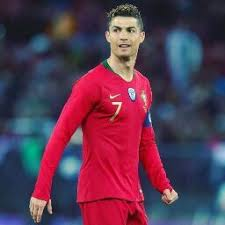
\includegraphics[width=\textwidth]{ronaldo.jpg}
            \caption*{ronaldo.jpg (Ronaldo)}
        \end{minipage}\hfill
        \begin{minipage}{0.48\textwidth}
            \centering
            
\includegraphics[width=\textwidth]{messi.jpg}
            \caption*{messi.jpg (Messi)}
        \end{minipage}
        \caption{Reusable JPEG MD5 collision: two different pictures with the same MD5 digest.}
        \label{fig:reusable-jpeg}
    \end{figure}

    \begin{lstlisting}[style=hashblock,caption={Hashes for the reusable JPEG pair}]
MD5(c1)    0edac4bf5802f193d4e2c64bdbf36671
MD5(c2)    0edac4bf5802f193d4e2c64bdbf36671
SHA256(c1) 22f2c829021e449455c27c15b28e7de8f1b24958606b39ca38af92429dc579ae
SHA256(c2) ed7a6e4d870f4f0035f1f7ecd5112d1065b817ad66bf95635fc24d8b5df6e1be
    \end{lstlisting}

    \begin{lstlisting}[style=textblock,
        caption={First difference \& prefix flips},
        label={lst:firstdiff}]
first diff @ byte 9 (0x9) : 00 -> 01
diffs inside 0..73:
  byte   9 : 00 -> 01
  byte  73 : 25 -> 24
    \end{lstlisting}

    Only two bytes differ in the 74-byte prefix; from byte~74~$\rightarrow$~EOF the files are identical.

    \begin{lstlisting}[style=textblock,
        caption={Identical suffix boundary \& length},
        label={lst:suffix}]
suffix starts at byte 74 (0x4A)
identical tail length = 16087 bytes
    \end{lstlisting}

    \begin{lstlisting}[style=textblock,
        caption={Steering flip (2nd COM length) and next-marker offsets},
        label={lst:comlength}]
COM@7 length: c1 = 119 (0x0077)   c2 = 375 (0x0177)
next-marker offsets from COM start (7): c1 -> 126   c2 -> 382
    \end{lstlisting}

    The flip at offset~9 changes the big-endian length of the second COM segment, moving where the next marker is parsed. This shift is sufficient to make one file display \emph{Messi} and the other \emph{Ronaldo} while preserving the same MD5.

    \begin{lstlisting}[style=hexhi,caption={collision1.jpg — first 96 bytes}]
00000000  ff d8 ff fe 00 03 aa ff fe @00@ 77 bb 82 c3 a6 dc  |..........w.....|
00000010  d8 0b eb a4 b3 fb f2 22 de 01 48 f7 85 1f 2f 63  |......."..H.../c|
00000020  52 df ef 06 9a 45 76 18 8b fd ea 25 13 57 83 4f  |R....Ev....%.W.O|
00000030  b6 23 6d fd 50 9b f2 2d 2f b7 d4 fe 85 da 23 e3  |.#m.P..-/.....#.|
00000040  ab b7 30 9c bc 5b 68 4c 61 @25@ 28 49 2e 18 b4 6d  |..0..[hLa%(I...m|
00000050  56 22 a2 b5 83 ab c4 97 0e fc 0f bd 68 dc e6 a0  |V"..........h...|
    \end{lstlisting}

    \begin{lstlisting}[style=hexhi,caption={collision1.jpg — first 96 bytes}]
00000000  ff d8 ff fe 00 03 aa ff fe @01@ 77 bb 82 c3 a6 dc  |..........w.....|
00000010  d8 0b eb a4 b3 fb f2 22 de 01 48 f7 85 1f 2f 63  |......."..H.../c|
00000020  52 df ef 06 9a 45 76 18 8b fd ea 25 13 57 83 4f  |R....Ev....%.W.O|
00000030  b6 23 6d fd 50 9b f2 2d 2f b7 d4 fe 85 da 23 e3  |.#m.P..-/.....#.|
00000040  ab b7 30 9c bc 5b 68 4c 61 @24@ 28 49 2e 18 b4 6d  |..0..[hLa$(I...m|
00000050  56 22 a2 b5 83 ab c4 97 0e fc 0f bd 68 dc e6 a0  |V"..........h...|
    \end{lstlisting}

    Visible flips: byte~9 \texttt{00$\rightarrow$01} (COM length high byte), byte~73 \texttt{25$\rightarrow$24} (small alignment tweak).

    \subsubsection{GZIP files}

    \paragraph{}
    GZIP members begin with a fixed header and optional fields (FEXTRA, FNAME, FCOMMENT). The reusable prefix lives in this flexible region (and around the start of the first DEFLATE stream). A one–byte flip in the crafted prefix shifts where the decompressor enters the subsequent member/blocks, yet the MD5 state after the prefix is equalized, so both files share the same MD5.

    \paragraph{Results.}
    Files:
    \begin{itemize}
        \item \texttt{collision1.tar.gz} size \textbf{1585} bytes
        \item \texttt{collision2.tar.gz} size \textbf{1585} bytes
    \end{itemize}

    \begin{lstlisting}[style=textblock, caption={Hashes for the reusable GZIP pair}, label={lst:gziphashes}]
MD5(c1)    ad2722dc523c28cc5eb865d9a08a2279
MD5(c2)    ad2722dc523c28cc5eb865d9a08a2279

SHA256(c1) 3633256c56b04a9da21156dfd3b128ef5aa4821aa62251e8974929be2f5fb5d2
SHA256(c2) 15cd07867f9c5a486bf14dab80f698e6a34ced64ac78c231e62882c8fa9ca357
    \end{lstlisting}

    \begin{lstlisting}[style=textblock, caption={Identical suffix boundary}, label={lst:gzip-suffix}]
suffix starts at byte 138 (0x8A)
identical tail length = 1447 bytes
    \end{lstlisting}

    \begin{lstlisting}[style=textblock, caption={GZIP headers (parsed)}, label={lst:gziphdr}]
header lengths: c1=52   c2=52
flags (c1/c2):  0x04 / 0x04
FNAME (c1/c2):  None / None
    \end{lstlisting}

    \begin{lstlisting}[style=hexhi, caption={GZIP prefix excerpt (visible flip)}, label={lst:gziphex}]
00000040  08 04 41 6e 67 65 02 ff 76 @00@ 43 42 72 00 2a 2a  |..Ange..v.CBr.**|
00000040  08 04 41 6e 67 65 02 ff 76 @01@ 43 42 72 00 2a 2a  |..Ange..v.CBr.**|
    \end{lstlisting}

    \textit{} A pair of single-bit flips occur inside the reusable prefix: at offset 0x49 (decimal 73) the byte changes \texttt{00$\rightarrow$01}, and at offset 0x89 (decimal 137) also changes. Because we use 0-based offsets, the identical suffix begins at byte 0x8A (decimal 138) = last flip + 1; from there to EOF the two files are byte-identical. Full per-format details are auto-generated in \texttt{techniques/reusable-format/gzip/out/analysis.md}.

    \subsubsection{PDF documents with different content}

    \paragraph{}
    PDF allows flexible object graphs and tolerates extra data. The crafted prefix sits before/around the first objects and tweaks a small piece of structure (e.g., which \texttt{/Pages} object the \texttt{/Catalog} references), so viewers render different documents even though MD5 is the same, and the remainder of the file is byte-identical.

    \paragraph{Results.}
    Files:
    \begin{itemize}
        \item \texttt{collision1.pdf} size \textbf{70634} bytes
        \item \texttt{collision2.pdf} size \textbf{70634} bytes
    \end{itemize}

    \begin{lstlisting}[style=textblock, caption={Hashes for the reusable PDF pair}, label={lst:pdfhashes}]
MD5(c1)    f4e3cebc927058950de2b46b0d5dfc38
MD5(c2)    f4e3cebc927058950de2b46b0d5dfc38

SHA256(c1) a191c6eae924038f52e89bbe62cda6236a2f5f97fcfa13fe86a9ead8d08be5fd
SHA256(c2) 51b7df6c065cb3b5d5e1cc6001cc23f6ce5e14a86c784b06ee14578048e2797c
    \end{lstlisting}

    \begin{lstlisting}[style=textblock, caption={Identical suffix boundary}, label={lst:pdf-suffix}]
suffix starts at byte 138 (0x8A)
identical tail length = 70496 bytes
    \end{lstlisting}

    \begin{lstlisting}[style=hexhi, caption={GZIP prefix excerpt (visible flip)}, label={lst:gziphex}]
00000040  5f 5f 2f 50 61 67 65 73 20 @32@ 20 30 20 52 0a 25  |__/Pages 2 0 R.%|
00000040  5f 5f 2f 50 61 67 65 73 20 @33@ 20 30 20 52 0a 25  |__/Pages 3 0 R.%|
    \end{lstlisting}

    \textit{} The small flip in the prefix changes the \texttt{/Catalog}’s \texttt{/Pages} reference (\texttt{2 0 R} $\rightarrow$ \texttt{3 0 R}), so viewers render different page trees. The suffix from byte~138 to EOF is identical in both files. Full per-format details are auto-generated in \texttt{techniques/reusable-format/pdf/out/analysis.md}.


    \paragraph{Reproducibility and artifacts.}
    All three reusable-collision experiments (JPEG, GZIP, PDF) are reproducible from our repository; each \texttt{run.sh} produces a pair of collided files and an \texttt{analysis.md} with hashes, first-difference locations, identical-suffix boundaries, and format-specific notes. See the per-format \texttt{out/} folders for the analysis files.

    \subsubsection{Applicability to Different File Formats}

    \paragraph{}
    While our experiments focused on JPEG, GZIP, and PDF, this reusable collision technique can be applied to other file formats that have flexible structures. For example, \textbf{PNG} is a good candidate because its 32-bit chunk lengths allow for large "jumps" over data, and viewers often ignore non-essential chunks. Similarly, \textbf{MP4} files use 32-bit and 64-bit "box" sizes, making it possible to skip large sections of the file by manipulating non-critical boxes like \texttt{free} or \texttt{skip}.

    \paragraph{}
    On the other hand, some file formats are difficult or impractical for this attack due to their rigid structures or the way they are parsed. These include:
    \begin{itemize}
        \item \textbf{GIF}: The data sub-blocks in a GIF have a maximum size of only 255 bytes (a 1-byte length). This makes it hard to “jump” over a large amount of data, and there is no known generic reusable collision method.
        \item \textbf{JPEG (with very large segments)}: The 16-bit length of a JPEG segment limits the maximum jump distance. Certain encoding methods also leave little room for inserting the necessary collision data.
        \item \textbf{ASN.1/DER (e.g., in \textit{strict} X.509)}: These formats have a strict structure where outer objects contain the total length of the inner objects. If an inner object's length is changed, the outer object's length becomes incorrect, making the entire file invalid.
        \item \textbf{Strict Parsers}: Some programs are written to be very strict and will reject a file if it contains unknown data or has extra data at the end. These parsers close the loophole that reusable prefix attacks depend on.
    \end{itemize}

    \newpage
    \section{Appendix A: Images, Graphs and Diagrams}

    \subsection{Complete Hexdump Visualization: Identical-Prefix Collision}

    Figure~\ref{fig:hexdump-full} shows the complete hexdump comparison of the identical-prefix collision experiment. The visualization displays both collision files side-by-side with difference markers:
    \begin{itemize}
        \item The readable ASCII prefix: \texttt{"02232\_Applied\_Cryptography\_Fall\_2025"}
        \item The 128-byte collision block with only 8 differing bytes (marked with 'X')
        \item The identical suffix containing the appendix text (all marked with '.')
    \end{itemize}

    This demonstrates how the Merkle-Damgård construction preserves collisions when identical suffixes are appended.

    \begin{figure}[p]
        \centering
        \includegraphics[page=1,width=0.95\textwidth]{hexdump_visualization.pdf}
        \caption{Complete hexdump comparison showing the structure of the identical-prefix MD5 collision. The rightmost column marks identical bytes with '.' and differing bytes with 'X'. Notice the concentration of differences in the collision block (bytes 0x40--0xBF) and the complete identity of the suffix (bytes 0xC0--EOF).}
        \label{fig:hexdump-full}
    \end{figure}

    \clearpage

    \subsection{Additional Diagrams}

    \begin{figure}
        \centering
        \includegraphics[width=1\linewidth]{X509Signing.drawio.png}
        \caption{Enter Caption}
        \label{fig:x509-signing}
    \end{figure}

    \begin{thebibliography}{99}

        \bibitem{albertini}
        Albertini, A. (n.d.). \textit{Hash Collisions and Exploitations}. GitHub repository. Available at: \url{https://github.com/corkami/collisions}

        \bibitem{fillinger2015}
        Fillinger, M., \& Stevens, M. (2015). Reverse-engineering of the cryptanalytic attack used in the Flame super-malware. In \textit{ASIACRYPT 2015}, LNCS 9453, pp. 586--611. Springer. Available at: \url{https://www.marc-stevens.nl/research/papers/AC15-FS.pdf}

        \bibitem{joux}
        Joux, A. (2004). Multicollisions in iterated hash functions. Application to cascaded constructions. In M. Franklin (Ed.), \textit{CRYPTO 2004}, LNCS 3152, pp. 306--316. Springer. Available at: \url{https://www-apr.lip6.fr/~jou/papers/2004_crypto_multicollisions.pdf}

        \bibitem{kelsey}
        Kelsey, J., \& Schneier, B. (2005). Second Preimages on n-bit Hash Functions for Much Less than $2^n$ Work. In R. Cramer (Ed.), \textit{EUROCRYPT 2005}, LNCS 3494, pp. 471--490. Springer. Available at: \url{https://www.schneier.com/academic/paperfiles/paper-preimages.pdf}

        \bibitem{klima}
        Klima, V. (2006). \textit{Tunnels in Hash Functions: MD5 Collisions Within a Minute}. Cryptology ePrint Archive, Report 2006/105. Available at: \url{https://eprint.iacr.org/2006/105}

        \bibitem{leurent2020}
        Leurent, G., \& Peyrin, T. (2020). \textit{SHA-1 is a Shambles: First Chosen-Prefix Collision on SHA-1 and Application to the PGP Web of Trust}. Cryptology ePrint Archive, Report 2020/014. Available at: \url{https://eprint.iacr.org/2020/014.pdf}

        \bibitem{microsoft}
        Microsoft. (2008). \textit{Microsoft Security Advisory 961509}. Available at: \url{https://learn.microsoft.com/en-us/security-updates/securityadvisories/2008/961509}

        \bibitem{nist}
        NIST NVD. (2009). \textit{CVE-2004-2761: MD5 not collision resistant}. Available at: \url{https://nvd.nist.gov/vuln/detail/CVE-2004-2761}

        \bibitem{rivest}
        Rivest, R. (1992). \textit{The MD5 Message-Digest Algorithm}. RFC 1321. Available at: \url{https://www.rfc-editor.org/rfc/rfc1321}

        \bibitem{stevens2009crypto}
        Stevens, M., Sotirov, A., Appelbaum, J., Lenstra, A., Molnar, D., Osvik, D. A., \& de Weger, B. (2009). Short chosen-prefix collisions for MD5 and the creation of a rogue CA certificate. In \textit{CRYPTO 2009}, LNCS 5677, pp. 55--69. Springer. Available at: \url{https://www.marc-stevens.nl/research/papers/CR09-SSALMOdW.pdf}

        \bibitem{stevens2012journal}
        Stevens, M., Lenstra, A., \& de Weger, B. (2012). Chosen-prefix collisions for MD5 and applications. \textit{International Journal of Applied Cryptography}, 2(4), pp. 322--359. Available at: \url{https://www.marc-stevens.nl/research/papers/IJACT12-StLdW.pdf}

    \end{thebibliography}

\end{document}